\documentclass{article}
\usepackage{iclr2027_conference,times}

\usepackage{hyperref}
\usepackage{url}
\usepackage{graphicx}
\usepackage{booktabs}
\usepackage{amsmath}
\usepackage{amssymb}
\usepackage{amsthm}
\usepackage{algorithm}
\usepackage{algpseudocode}
\usepackage{tikz}
\usetikzlibrary{arrows.meta,positioning,fit,backgrounds,calc}
\urlstyle{rm}

\newtheorem{definition}{Definition}
\newtheorem{proposition}{Proposition}

\newcommand{\fix}{\marginpar{FIX}}
\newcommand{\new}{\marginpar{NEW}}

% -----------------------------------------------------------------------
\title{CutWorld: A Latent Dynamics Model for Unified Branch-and-Cut Control}

% Authors must not appear in the submitted version.
% \author{...}

% \iclrfinalcopy  % Uncomment for camera-ready version only
% -----------------------------------------------------------------------

\begin{document}

\maketitle

\begin{abstract}
Modern Mixed-Integer Programming solvers rely on Branch-and-Cut, which must
make sequential decisions: which variable to branch on, which cuts to add,
which node to explore, at every step of an exponentially large search tree.
Because each decision reshapes the subsequent search, methods that score
candidates from the current node alone are blind to the very signal that makes
their target expert, strong branching, effective. We present CutWorld, a latent dynamics model that learns to simulate the downstream consequences of
Branch-and-Cut decisions in latent space, replacing expensive LP solves with a
single cheap forward pass. Our model encodes each search node as a bipartite
graph using a GATv2 network with learned cross-attention pooling, then rolls
forward a causal Transformer to predict how both the global state and each
variable's representation evolve under a candidate action, enabling the
branching policy to be re-applied to imagined states for multi-step planning.
Candidates are scored by a MuZero-style return combining predicted per-step
rewards, a value estimate, and a cost-to-go penalty; the same latent drives
Gomory cut selection and node ordering within a single unified model that
provably preserves solver exactness. On medium-tier Set Cover ($500{\times}1000$, 300\,s budget), every neural
variant terminates on all instances while every classical branching rule in the
same harness times out; a single-step latent rollout reduces explored nodes by
44\% over the imitation policy (SGM 3{,}197 vs.\ 5{,}733), and deeper rollout
(depth\,3) increases nodes by 14\%, confirming that short-horizon planning is
the correct regime given current dynamics fidelity. We evaluate across medium and
hard tiers against SCIP, pseudocost, strong branching, and classical heuristics,
reporting optimality rate, nodes explored, wall-clock solving time, and cuts
applied, with component-wise ablations isolating the contribution of each element.
\end{abstract}

% -----------------------------------------------------------------------
\section{Introduction}

A modern optimization solver is, at its core, a sequential decision maker. To
solve a single instance it makes millions of discrete choices --- which variable
to branch on, which cutting planes to add, which open node to explore next ---
each one steering an enormous combinatorial search, and each governed today by a
hand-engineered heuristic. Model-based planning agents such as MuZero and
Dreamer \citep{schrittwieser2020mastering,hafner2020dream} have shown that
learning a model of environment dynamics, and planning by imagining the
consequences of actions, transforms sequential decision making, from Atari and
Go to continuous control. We bring this idea inside an optimization solver:
\emph{CutWorld}, a latent dynamics model for the solver's most consequential
decisions, those of Branch-and-Cut.

Mixed-Integer Programming (MIP) is a cornerstone of combinatorial optimization,
and modern solvers attack it with Branch-and-Cut. Starting from a linear
programming (LP) relaxation, B\&C repeatedly executes two core operations at
each search tree node: adding cutting planes, valid inequalities that tighten
the relaxation without removing integer solutions, and branching on a fractional
variable to partition the search space.

Unfortunately, making high-quality decisions at every node is computationally
expensive. The gold standard for branching, \emph{strong branching}, tentatively
solves the child LPs of each candidate variable to measure its bound
improvement; cut selection faces an analogous trade-off when choosing among
large pools of valid inequalities. To amortize these costs, recent machine
learning approaches learn to imitate strong branching in a single forward pass,
e.g., with graph neural networks \citep{gasse2019exact,khalil2016learning}, or
use reinforcement learning to select cuts \citep{tang2020reinforcement}. These
methods are effective, but they share a structural limitation: each scores a
candidate \emph{from the current node alone}, discarding the lookahead
signal --- the effect a decision has on the resulting subtree.

CutWorld closes this gap with a learned latent dynamics model that simulates the
immediate consequences of candidate decisions in latent space, without
executing child LP solves. We encode each search node as a bipartite graph,
reading out the graph-level state with a learned attention pool
\citep{lee2019set} over variable embeddings that emphasizes structurally
important variables rather than averaging uniformly, and train a causal
Transformer \citep{teoh2024nextlatent} to predict how this state, alongside its
constituent per-variable embeddings, evolves under a candidate branching
action. Because the model predicts fine-grained, per-variable representations
rather than a static graph summary, the branching policy can be re-applied to
the imagined child state for a one-step latent lookahead. Candidates are scored
by combining the predicted child node's dual-bound value with a learned
subtree-size penalty that directly targets the solver's true cost in explored
nodes. Cut selection follows a similar imitation-learning approach
\citep{paulus2022learning}, scoring candidate Gomory cuts with a pointer
network conditioned on the current search state. A single unified model
concurrently drives the solver's core discrete choices --- variable branching,
cut selection, and node ordering --- influencing only which decisions the solver
makes and in what order, never the bounds or feasibility tests, so exactness is
preserved.

\paragraph{Summary of Contributions.}
\begin{itemize}
  \item \textbf{A latent dynamics model for Branch-and-Cut.} We learn a
  solver's decision dynamics --- the first instance of \emph{latent dynamics
  models for optimization} --- so that branching and cutting are \emph{planned
  in imagination} rather than chosen by fixed heuristics, replacing the child
  LP solves that strong branching requires with a single learned latent
  transition per candidate.

  \item \textbf{Unified control with exactness guarantees.} We show that a
  single latent model can simultaneously drive variable branching, node
  selection, and cut selection while strictly maintaining the solver's
  exact optimality guarantees.

  \item \textbf{A search-tailored objective and stable training.} We design a
  subtree-size prediction objective targeting the solver's true cost --- total
  explored nodes --- trainable directly from non-depth-first search traces,
  stabilized via latent overshooting with a grounded bound-prediction
  auxiliary.

  \item \textbf{Empirical validation.} On Set Cover across difficulty tiers we
  report the four metrics that determine solver quality: optimality, explored
  nodes, solving time, and cuts applied, with an ablation that isolates each
  planning component's contribution and a fair both-solved-subset comparison
  against SCIP and classical branching heuristics.
\end{itemize}

% -----------------------------------------------------------------------
\section{Related Work}

Learning to make solver decisions is an active area \citep{bengio2021machine}.
The dominant approach is imitation: \citet{khalil2016learning} regress
strong-branching scores from hand-crafted features, and \citet{gasse2019exact}
represent a node as a bipartite constraint--variable graph and train a graph
network to imitate strong branching in a single forward pass. This amortizes the
cost of strong branching but discards the very signal that makes it strong ---
the quality of the subtree each candidate ultimately induces. The bipartite
encoder of \citet{gasse2019exact} is the node representation we build on; we
replace its global mean pooling with a learned attention readout
\citep{lee2019set} over variable nodes, producing a graph-level state that
emphasizes fractional and high-objective variables rather than averaging
uniformly. Reinforcement learning restores a longer horizon:
\citet{scavuzzo2022learning} train a branching policy with tree-structured
returns, and \citet{nair2020solving} scale neural MIP solving with learned
diving and branching. These methods optimize long-term reward, but remain
\emph{model-free}: they treat the solver as a black box and never learn how a
decision reshapes the subsequent search state. The theoretical conditions under
which learned branching rules preserve solver correctness are studied by
\citet{chengbasu2023theoretical}, motivating our design that gates all learned
decisions behind bound-justified pruning rather than letting them alter
feasibility or optimality tests. Graph neural networks have also been applied
directly to Set Cover \citep{shafi2022graphscp}, the benchmark domain we
evaluate on.

Cut selection has been learned along the same lines. \citet{tang2020reinforcement}
cast it as a sequential decision problem solved with reinforcement learning, and
\citet{paulus2022learning} imitate a look-ahead expert that scores each cut by
the bound improvement it yields, but the look-ahead only produces training
labels; at inference the policy again predicts from the current node alone.
\citet{wang2023hierarchical} model cut selection as a sequential ranking
problem with a hierarchical sequence model; like prior cut methods, selection
is made from the current node without imagining downstream states. Learned
large neighborhood search \citep{sonnerat2021learning} targets yet another
solver decision. Across branching and cutting alike, prior work scores a
candidate either myopically or through an explicit, expensive look-ahead that
the learned policy itself cannot invoke.

CutWorld instead draws on model-based reinforcement learning. MuZero
\citep{schrittwieser2020mastering} plans with a learned dynamics model without
reconstructing observations, and Dreamer \citep{hafner2020dream} learns
behaviors by imagination in latent space. Recent work on compact world models
\citep{teoh2024nextlatent} shows that predicting next latents in a learned
embedding space, rather than reconstructing raw observations, yields efficient
and accurate forward models; our DynamicsTransformer follows this design, and
we adopt latent overshooting as a training-time stabilizer to keep the learned
forward model faithful across multiple steps even though the deployed solver
plans with a single-step rollout. We bring this inside Branch-and-Cut,
combining the bipartite representation of \citet{gasse2019exact} with a
learned latent forward model: rather than ranking candidates by a static score
or paying for explicit LP look-ahead, we \emph{imagine} the immediate
consequence a decision induces and recover part of strong branching's
look-ahead signal at the cost of a single cheap latent transition per
candidate. A single such model drives branching, cut selection, and node
ordering, whereas prior methods learn each decision in isolation.

% -----------------------------------------------------------------------
\section{Background and Problem Formulation}

A (binary) Mixed-Integer Program minimizes a linear objective over integer
variables subject to linear constraints,
\begin{equation}
  \min_{x}\ c^\top x \quad \text{s.t.}\quad Ax \ge b,\quad x \in \{0,1\}^n,
\end{equation}
with $c\in\mathbb{R}^n$, $A\in\mathbb{R}^{m\times n}$, $b\in\mathbb{R}^m$.
Set Cover is the case $A\in\{0,1\}^{m\times n}$, $b=\mathbf{1}$.

Branch-and-Cut solves the LP relaxation at each node; if the solution is
fractional it either adds valid cutting planes $\alpha^\top x \ge \beta$ that
tighten the relaxation, or branches on a fractional variable $x_j$ into the
subproblems $x_j=0$ and $x_j=1$. The number of nodes explored before optimality
is proved is governed by these two choices.

We model the search as an MDP $(\mathcal{S},\mathcal{A},P,R,\gamma)$: a state
$s_t$ is a search node (its LP relaxation as a constraint--variable graph); an
action $a_t$ selects a fractional variable to branch on or a cut to add; the
transition $P$ is the solver's deterministic response (child LPs, tightened
relaxation); and the per-step reward $r_t$ is the dual-bound improvement, a
dense proxy for progress. The ultimate objective is to prove optimality in as
few explored nodes as possible.

The transition $P$ is realized by the solver itself, solving child LPs and
re-optimizing, so evaluating the downstream effect of an action costs as much as
taking it, which is why prior learned policies avoid look-ahead. CutWorld's
central idea is to learn a latent surrogate for $P$: an encoder maps states to a
latent, and a learned dynamics model predicts how that latent transitions under
an action, so a decision's consequences can be \emph{imagined} without invoking
the solver. This turns look-ahead from an expensive oracle into a cheap forward
pass, and the reward and node-count signals above become the learning targets for
the model's reward and cost-to-go heads (Section~\ref{sec:method}).

\label{sec:exactness}
\begin{proposition}[Exactness]
\label{prop:exact}
For any branching variable chosen among the fractional candidates, any subset of
globally valid cuts added at any node, and any ordering of the open nodes,
Branch-and-Cut returns a global optimum. Consequently CutWorld preserves the
solver's exactness guarantee for every setting of the learned policy.
\end{proposition}
\begin{proof}[Proof sketch]
Branching on a fractional $x_j$ into $x_j=0$ and $x_j=1$ partitions the
integer feasible set exhaustively, so no integer solution is lost. A globally
valid cut is satisfied by every integer-feasible point, so adding it removes no
feasible solution. Node ordering changes only the sequence in which subproblems
are explored, not the bound-and-integrality pruning rule, hence not the final
incumbent. The learned model only selects among these correctness-preserving
options, so the incumbent at termination is a global optimum.
\end{proof}

Our validity requirement drives the cut design in Section~\ref{sec:method}: we
generate Gomory fractional cuts, which are valid by construction, and let the
model \emph{select} among them rather than invent inequalities.

% -----------------------------------------------------------------------
\section{Method}
\label{sec:method}

\begin{figure*}[t]
\centering
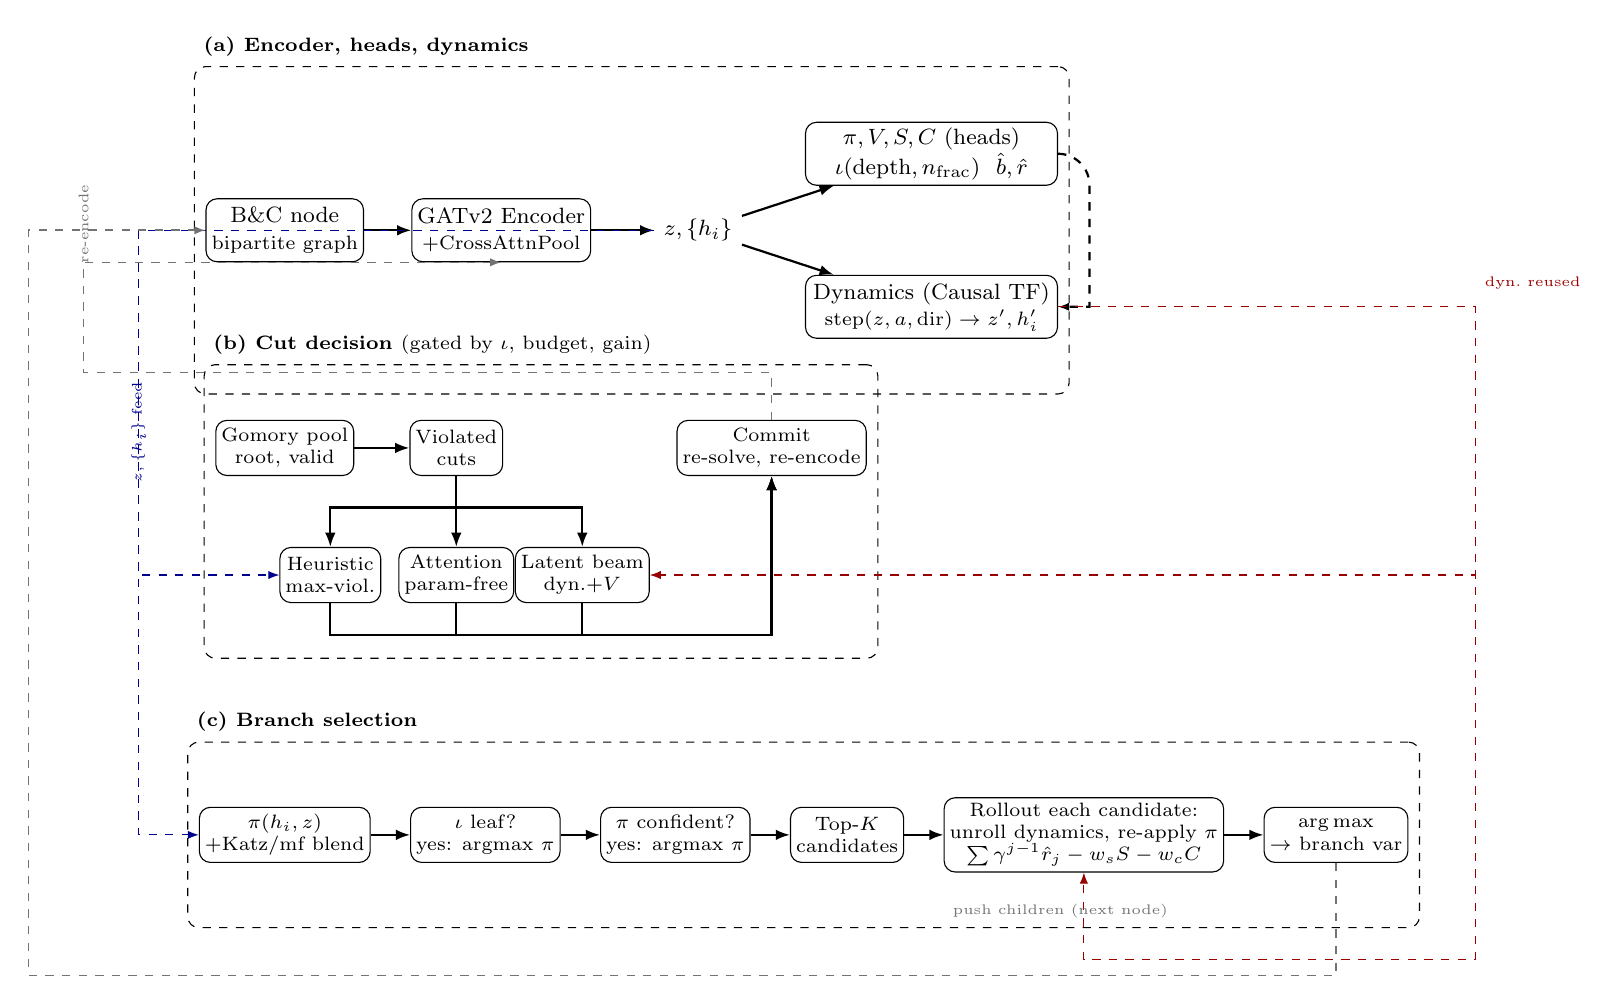
\begin{tikzpicture}[
  node distance=4mm and 6mm,
  box/.style={draw, rounded corners, align=center, minimum height=8mm,
              inner sep=2pt, font=\footnotesize},
  small/.style={draw, rounded corners, align=center, minimum height=7mm,
              inner sep=2pt, font=\scriptsize},
  lat/.style={align=center, font=\footnotesize},
  panel/.style={draw, dashed, rounded corners, inner xsep=4pt, inner ysep=7mm},
  ptitle/.style={font=\scriptsize\bfseries, anchor=south west},
  arr/.style={-{Latex[length=1.8mm]}, thick},
  thinarr/.style={-{Latex[length=1.4mm]}},
  feed/.style={thinarr, dashed, blue!55!black},
  reuse/.style={thinarr, dashed, red!60!black},
  loop/.style={thinarr, dashed, black!55, line width=0.6pt},
]

% ---------- Panel (a): core architecture ----------
\node[box] (inp) {B\&C node\\{\scriptsize bipartite graph}};
\node[box, right=of inp] (enc) {GATv2 Encoder\\{\scriptsize +CrossAttnPool}};
\node[lat, right=8mm of enc] (z) {$z,\{h_i\}$};
\node[box, above right=3mm and 8mm of z, minimum width=32mm] (heads)
  {$\pi,V,S,C$ (heads)\\$\iota(\text{depth},n_{\text{frac}})$\ \ $\hat b,\hat r$};
\node[box, below right=3mm and 8mm of z, minimum width=32mm] (dyn)
  {Dynamics (Causal TF)\\{\scriptsize step$(z,a,\text{dir})\to z',h_i'$}};

\draw[arr] (inp) -- (enc);
\draw[arr] (enc) -- (z);
\draw[arr] (z) -- (heads);
\draw[arr] (z) -- (dyn);
\draw[arr, thinarr, dashed] (heads.east) to[out=0,in=90] ++(4mm,-4mm) |- (dyn.east);

\node[panel, fit=(inp)(enc)(z)(heads)(dyn)] (panelA) {};
\node[ptitle] at (panelA.north west) {(a) Encoder, heads, dynamics};

% ---------- Panel (b): cut decision ----------
\node[small, below=20mm of inp] (pool) {Gomory pool\\{\scriptsize root, valid}};
\node[small, right=7mm of pool] (viol) {Violated\\cuts};
\node[small, below=9mm of viol, xshift=-16mm] (heur) {Heuristic\\{\scriptsize max-viol.}};
\node[small, below=9mm of viol] (attn) {Attention\\{\scriptsize param-free}};
\node[small, below=9mm of viol, xshift=16mm] (latent) {Latent beam\\{\scriptsize dyn.+$V$}};
\node[small, right=22mm of viol] (commit) {Commit\\{\scriptsize re-solve, re-encode}};

\draw[arr] (pool) -- (viol);
\draw[arr] (viol.south) -- ++(0,-4mm) -| (heur.north);
\draw[arr] (viol.south) -- (attn.north);
\draw[arr] (viol.south) -- ++(0,-4mm) -| (latent.north);
\draw[arr] (heur.south) -- ++(0,-4mm) -| (commit.south);
\draw[arr] (attn.south) -- ++(0,-4mm) -| (commit.south);
\draw[arr] (latent.south) -- ++(0,-4mm) -| (commit.south);

\node[panel, fit=(pool)(viol)(heur)(attn)(latent)(commit)] (panelB) {};
\node[ptitle] at (panelB.north west) {(b) Cut decision\ {\normalfont\scriptsize(gated by $\iota$, budget, gain)}};

% ---------- Panel (c): branch selection ----------
\node[small, below=42mm of pool] (pscore) {$\pi(h_i,z)$\\{\scriptsize +Katz/mf blend}};
\node[small, right=5mm of pscore] (leafchk) {$\iota$ leaf?\\{\scriptsize yes: argmax $\pi$}};
\node[small, right=5mm of leafchk] (confchk) {$\pi$ confident?\\{\scriptsize yes: argmax $\pi$}};
\node[small, right=5mm of confchk] (topk) {Top-$K$\\candidates};
\node[small, right=5mm of topk, minimum width=30mm] (roll)
  {Rollout each candidate:\\unroll dynamics, re-apply $\pi$\\
   $\sum\gamma^{j-1}\hat r_j - w_sS - w_cC$};
\node[small, right=5mm of roll] (argmax) {$\arg\max$\\$\to$ branch var};

\draw[arr] (pscore) -- (leafchk);
\draw[arr] (leafchk) -- (confchk);
\draw[arr] (confchk) -- (topk);
\draw[arr] (topk) -- (roll);
\draw[arr] (roll) -- (argmax);

\node[panel, fit=(pscore)(leafchk)(confchk)(topk)(roll)(argmax)] (panelC) {};
\node[ptitle] at (panelC.north west) {(c) Branch selection};

% ---------- Cross-panel interconnections ----------
\coordinate (rbus) at ($(panelC.east)+(7mm,0)$);
\draw[reuse] (dyn.east) -- (dyn.east -| rbus)
             -- (latent.east -| rbus) -- (latent.east);
\draw[reuse] (dyn.east) -| (rbus |- panelC.south) -- ++(0,-4mm) -| (roll.south);
\node[font=\tiny, red!60!black, anchor=west] at ($(dyn.east -| rbus)+(0,3mm)$) {dyn.\ reused};

\coordinate (lbus) at ($(panelA.west)+(-7mm,0)$);
\draw[feed] (z.west) -- (z.west -| lbus)
            -- (heur.west -| lbus) -- (heur.west);
\draw[feed] (z.west -| lbus) -- (pscore.west -| lbus) -- (pscore.west);
\node[font=\tiny, blue!55!black, anchor=east, rotate=90] at ($(lbus)+(0,-18mm)$) {$z,\{h_i\}$ feed};

\coordinate (lbus2) at ($(panelA.west)+(-14mm,0)$);
\coordinate (commitN) at ($(commit.north)+(0,6mm)$);
\draw[loop] (commit.north) -- (commitN) -- (commitN -| lbus2)
            -- (enc.south -| lbus2) -- (enc.south);
\node[font=\tiny, black!55, anchor=east, rotate=90] at ($(lbus2)+(0,7mm)$) {re-encode};

\coordinate (fbus) at ($(panelA.west)+(-21mm,0)$);
\coordinate (bbus) at ($(panelC.south)+(0,-6mm)$);
\draw[loop] (argmax.south) -- (argmax.south |- bbus)
            -- (fbus |- bbus) -- (fbus |- inp.west) -- (inp.west);
\node[font=\tiny, black!55, anchor=north] at ($(argmax.south)+(-35mm,-4mm)$) {push children (next node)};

\end{tikzpicture}
\caption{\textbf{CutWorld architecture and decision pipeline.}
\textbf{(a)} A GATv2 encoder with cross-attention pooling maps each
Branch-and-Cut node to a graph latent $z$ and per-variable embeddings
$\{h_i\}$; seven heads read $z$ (four also read $\{h_i\}$), and a causal
Transformer predicts how $z$ and $\{h_i\}$ evolve under a candidate action,
without invoking the solver. \textbf{(b)} Cut selection is gated by the
integrality head $\iota$ together with budget/gain/depth checks (Gate~7);
candidate Gomory cuts are scored by one of three interchangeable rules ---
maximum violation, a parameter-free attention rule over cut and constraint
embeddings, or a learned latent beam search over the dynamics --- before the
chosen cuts are committed and the LP is re-solved and re-encoded.
\textbf{(c)} Branching scores fractional variables with the policy head
$\pi$ (optionally blended with Katz centrality or fractionality); the
integrality head and the policy's own confidence provide two cheap early
exits, and only otherwise-ambiguous nodes pay for a latent rollout that
unrolls the dynamics, re-applies $\pi$ at each imagined step, and scores
candidates by a reward-, size-, and cost-to-go-weighted return.
\textbf{Cross-panel links} make the shared machinery explicit: the blue
dashed path shows $z,\{h_i\}$ from the encoder feeding both the cut-scoring
cluster and the branching policy; the red dashed path shows the dynamics
model being reused by the latent-beam cut mode and by the branch rollout;
and the two gray dashed loops close the search loop --- committing cuts
re-solves the LP and re-encodes a fresh $z,\{h_i\}$ (top loop), and the
chosen branch variable's children are pushed back onto the queue as new
B\&C nodes (bottom loop). No gate or head ever alters an LP bound or a
feasibility test, so solver exactness is unaffected
(Proposition~\ref{prop:exact}).}
\label{fig:arch}
\end{figure*}

We view Branch-and-Cut as a sequential decision process. At each node $t$ of
the search the solver observes a state $s_t$ (the current relaxation), takes an
action $a_t$ (branch on a fractional variable, or add a cut), and transitions to
the next node. We learn (i)~an encoder that maps $s_t$ to a latent state,
(ii)~a dynamics model that predicts how that latent evolves under an action, and
(iii)~heads that score decisions by rolling the dynamics forward
(Figure~\ref{fig:arch}). Throughout, $d=128$ denotes the embedding dimension.

\subsection{Node Encoder}

Each node is a bipartite graph over the constraints and variables of the
relaxation: variable nodes carry 19 LP-derived features (solution value,
fractionality, reduced cost, bound and basis status), constraint nodes carry 5
features (zero-padded to 19 in a shared feature matrix), and each edge carries
its coefficient together with two derived features, the RHS-normalized value and
the sign. A 3-layer bidirectional GATv2 network \citep{brody2022how} with 4
attention heads (head dimension 32, concatenated to $d=128$) performs
two-directional message passing per layer --- constraints-to-variables and
variables-to-constraints --- with LayerNorm after each pass. GATv2 attention,
rather than mean aggregation, lets each variable weight the constraints that
actually bind it at the current node, which vary enormously across the tree.
A learned cross-attention readout (CrossAttentionPool) attends a single learned
query vector over the per-variable embeddings to produce the graph-level
summary, emphasising the variables most relevant at this node:
\begin{equation}
  \bigl(\{h_i\}_{i=1}^{n},\, z\bigr) = \mathrm{Enc}(s_t),
  \qquad h_i,\, z \in \mathbb{R}^{d}.
\end{equation}
Feature statistics are held in fixed registered buffers rather than BatchNorm,
so the encoder can be frozen during later curriculum phases without any
train/eval inconsistency. The embedding of an action that branches on variable
$v$ is $a = h_v$.

\subsection{Latent Dynamics}

A 4-layer causal Transformer with 4 attention heads, hidden dimension $d=128$,
FFN width $4d$, maximum sequence length 512, and learned positional encodings
models the evolution of the latent along the root-to-node trajectory. Each step
produces one token encoding the current latent, the branched variable, and the
branch direction:
\begin{equation}
  u_\tau = W_{\mathrm{in}}[z_\tau \,\|\, a_\tau \,\|\, d_\tau],
  \quad \tau \le t,
\end{equation}
where $a_\tau = h_{v_\tau}$ is the embedding of the branched variable and
$d_\tau \in \{+1,-1\}$ is the branch direction. Conditioning on direction is
what lets a single model represent both children of a node. The next graph
latent is decoded with a residual connection to limit multi-step drift:
\begin{equation}
  z_{t+1} = \mathrm{LN}\!\bigl(z_t + W_{\mathrm{out}}\,\mathrm{TF}(u_{0:t})\bigr).
\end{equation}
Predicting a delta rather than an absolute latent keeps long rollouts from
wandering. A per-variable module predicts how each variable embedding evolves.
Exploiting the linearity of its first layer, the update decomposes as
\begin{equation}
  h_i^{\,t+1} = \mathrm{LN}\!\bigl(
    h_i^{\,t} + W_h(h_i^{\,t}) + W_z(z_{t+1}) + W_a(a_t)
  \bigr),
  \label{eq:varupdate}
\end{equation}
where $W_h$, $W_z$, $W_a$ are linear maps. Because $W_z(z_{t+1})$ and
$W_a(a_t)$ are identical across variables, they are computed once and
broadcast-added to the per-variable term $W_h(h_i^{\,t})$, reducing the
per-step cost from $O(V{\cdot}3d^2)$ to $O(V{\cdot}d^2)$. Predicting
per-variable embeddings~\eqref{eq:varupdate}, rather than only the graph
summary $z$, is what lets the branching policy be re-applied to an
\emph{imagined} state during planning. We ground the latent with a linear head
$\hat{b}_{t+1}=w_b^\top z_{t+1}$ that predicts the node's normalized dual
bound, tying the imagined latent to a real solver quantity, and a reward head
$\hat{r}_{t}=w_r^\top z_{t+1}$ that predicts the per-step dual-bound
improvement.

\subsection{Value, Cost-to-Go, and Policy}

Let $\bar{h}_{\mathrm{frac}}$ be the mean embedding of the \emph{currently
fractional} variables only. The value and cost-to-go heads share this enriched
input, so each head sees what is actually undecided at this node rather than a
global average:
\begin{align}
  V(z) &= \mathrm{MLP}_V([z \,\|\, \bar{h}_{\mathrm{frac}}]), \\
  C(z) &= \mathrm{softplus}\bigl(\mathrm{MLP}_C([z \,\|\,
           \bar{h}_{\mathrm{frac}}])\bigr),
\end{align}
where each MLP has layers $2d \to d \to d/2 \to 1$ and $C$ predicts
$\log(1+\text{remaining nodes})$. Its regression target is the Monte-Carlo
return $T-t$ read directly off a length-$T$ trajectory --- the number of steps
still to come, which requires \emph{no} assumption that the trajectory is
depth-first ordered, unlike a subtree-size target. The branching policy is a
pointer network scoring each fractional variable jointly against the graph
context:
\begin{equation}
  \pi(v) \propto w^\top\!\tanh\!\bigl(W_k h_v + W_z z\bigr)
                 \odot W_q z \,/\, \sqrt{d}.
\end{equation}
An integrality head $\sigma\!\bigl(\mathrm{MLP}([z \,\|\, \mathrm{depth} \,\|\,
n_{\mathrm{frac}}])\bigr)$ predicts the probability that the next node is a
leaf, used to gate the rollout (skip if already near-integral) and to control
when the cut pipeline fires.

\subsection{Planning Rollout for Candidate Selection}

To branch, we take the policy's top-$k$ candidates and score each by imagining
the subtree it induces. Starting from the current $(z,\{h_i\})$ with first
action $a=h_c$, we unroll the dynamics for $K$ steps, re-applying the policy to
each predicted state to choose the next action
$v_j=\arg\max_{v\in\mathcal{F}}\pi(v\mid z_j,\{h^j\})$ over the fractional set
$\mathcal{F}$. The candidate is scored by a MuZero-style return that accumulates
predicted rewards along the imagined path, bootstraps with the value at the
leaf, and penalizes predicted remaining work:
\begin{equation}
  R(c) = \sum_{j=1}^{K}\gamma^{\,j-1}\hat{r}_j
       + \gamma^{\,K-1}V(z_K)
       - w_c\sum_{j=1}^{K}\gamma^{\,j-1}\hat{C}(z_j).
  \label{eq:return}
\end{equation}
We expand a shallow tree of branching factor $b$ (the top-$b$ actions at each
step, child returns averaged); $b\!=\!1$ recovers a single greedy rollout.
Rather than branching on $\arg\max_c R(c)$, which lets a single noisy rollout
override a confident policy, we use a \emph{policy-anchored} rule: over the
candidate set we standardize the policy scores and the returns and select
$c^\star=\arg\max_c\bigl[\hat{\pi}(c)+\lambda\,\hat{R}(c)\bigr]$, so the
latent lookahead refines the policy's ranking instead of replacing it
($\lambda\!=\!0$ recovers the policy). A short horizon is used because deeper
rollouts compound dynamics error, and the rollout is invoked only when the
policy is uncertain; if the top candidate's probability exceeds a threshold the
policy choice is taken directly, so the lookahead cost is paid only on
genuinely close decisions. The same value drives \emph{node selection}: open
nodes are ordered by ascending predicted cost-to-go $C(z)$, so the subtree
expected to close soonest is explored first. Because these choices affect only
search order, never the bounds or feasibility tests, exactness is preserved.
Algorithm~\ref{alg:select} summarizes candidate selection.

\begin{algorithm}[t]
\caption{Branching-variable selection by latent rollout}
\label{alg:select}
\begin{algorithmic}[1]
\State \textbf{Input:} node latent $z$, variable embeddings $\{h_i\}$,
       fractional set $\mathcal{F}$, depth $K$, factor $b$
\State $\mathcal{C}\gets \textsc{TopK}_k\bigl(\pi(\cdot\mid z,\{h_i\}),\,\mathcal{F}\bigr)$
\For{each candidate $c\in\mathcal{C}$}
  \State $R(c)\gets \textsc{Rollout}(z,\{h_i\},c,K,b)$
         \Comment{Eq.~\eqref{eq:return}}
\EndFor
\State \Return $\arg\max_{c\in\mathcal{C}} R(c)$
\end{algorithmic}
\end{algorithm}

\subsection{Cutting-Plane Selection}

The model performs cut \emph{selection}; validity is guaranteed by the
generator, not the learner. We generate a pool of Gomory fractional cuts at the
root from the LP optimal basis. Writing the relaxation in standard form --- all
variables nonneg\-ative, with the box $0\le x\le 1$ lifted into explicit rows
$x_j+t_j=1$ so every nonbasic variable rests at its lower bound --- each basic
structural variable $x_j$ with a fractional value $\bar{b}$ and tableau row
$x_j+\sum_{k\in\mathcal{N}}\alpha_k v_k=\bar{b}$ yields the valid inequality
$\sum_{k\in\mathcal{N}}\mathrm{frac}(\alpha_k)\,v_k \ge \mathrm{frac}(\bar{b})$,
which we express in the structural variables by substituting the slack
definitions. Derived from globally valid rows with no branching bounds applied,
these cuts hold for \emph{every} integer-feasible solution and are safely
inherited by all descendants of the node --- genuine Branch-and-Cut rather than
cut-and-branch.

A pointer head scores each candidate cut $\ell$ against the node latent. Each
cut is represented by a 6-dimensional feature vector $\phi_\ell$ encoding
violation, efficacy, density, parallelism, objective cutoff, and support
fraction:
\begin{equation}
  \rho_\ell = w^\top\tanh\!\bigl(W_k\,\mathrm{MLP}(\phi_\ell)+W_z z\bigr),
\end{equation}
and cuts with $\sigma(\rho_\ell)>\tau$ are added, replacing fixed heuristics
such as maximum violation. As a parameter-free fallback, cuts and constraints
are each embedded as coefficient-weighted sums of $\{h_i\}$ over their
variable support, and cuts are scored by their cross-attention alignment with
constraints that are simultaneously loose and connected to fractional variables
--- a geometrically grounded selection rule that exploits the encoder's
representations without any additional learned parameters. Training the
pointer head requires cut-quality labels produced by an external solver, which
are not always available at the scale needed for Phase~5; the reported results
therefore use the attention rule as the deployed selection mechanism, with the
learned pointer head evaluated separately in Table~\ref{tab:cuts}.

\subsection{Learning Objectives}
\label{sec:objectives}

Each component has a supervised objective, optimized in the five-phase
curriculum detailed in Section~\ref{sec:training}:
\begin{itemize}
  \item \textbf{Policy:} a convex combination
  $\alpha\,\mathrm{CE}(\arg\max)+(1{-}\alpha)\,\mathrm{KL}(p_{\mathrm{SB}}\,\|\,\pi)$,
  $\alpha=0.5$, of hard cross-entropy against the strong-branching argmax and a
  soft KL term against $p_{\mathrm{SB}}=\mathrm{softmax}$ of the (per-node
  standardized) strong-branching scores; the hard term anchors the top-1
  choice while the soft term carries the full ranking signal.
  \item \textbf{Value:} Huber loss against the normalized dual bound.
  \item \textbf{Dynamics:} an MSE-plus-cosine loss on the one-step latent
  prediction $z_{t+1}$; an analogous MSE-plus-cosine reconstruction loss on
  $h_i^{\,t+1}$; Huber grounding losses on the two auxiliary heads $\hat{b}$
  (normalized dual bound) and $\hat{r}$ (per-step reward); and a
  \emph{latent-overshooting} loss that re-derives the same terms from the
  model's own free-running predictions over a horizon ramped from 1 to 3 steps
  across training, weighted by $1/k$, to curb compounding error.
  \item \textbf{Cost-to-go:} Huber loss on $\log(1{+}(T{-}t))$, where the
  target $T-t$ is the Monte-Carlo number of steps remaining in the trajectory.
  \item \textbf{Subtree size:} Huber loss on $\log(1{+}\text{subtree size})$
  from realized Branch-and-Cut traces; used during joint fine-tuning to shape
  the rollout's size penalty rather than as a standalone solver-time signal.
  \item \textbf{Integrality:} weighted binary cross-entropy against a
  leaf/non-leaf label, with positive-class weight equal to the
  negative-to-positive ratio.
  \item \textbf{Value-consistency} (joint phase only): $\lVert
  V(\tilde{z})-V(z)\rVert^2$, aligning the value head's output on the
  dynamics-predicted latent $\tilde{z}$ to its output on the true encoder
  latent $z$ for the same node, so $V$ stays reliable when queried on imagined
  states during planning.
  \item \textbf{Cutting-plane head:} weighted binary cross-entropy against a
  label indicating whether a candidate cut was selected by an external solver
  and improved the LP bound; positive-class weight equal to the
  negative-to-positive ratio.
\end{itemize}

% -----------------------------------------------------------------------
\section{Experiments}

\subsection{Setup}

We evaluate on Set Cover instances across easy, medium, and hard difficulty
tiers, collecting strong-branching trajectories for training. We compare against
a spectrum of branching rules: the trivial \emph{most-fractional} heuristic,
\emph{classical strong branching} at look-ahead depths 1, 4, and 8 (SB-1/4/8),
and \emph{SCIP}'s default reliability-pseudocost branching (the strong solver
baseline). We also report the \emph{imitation} policy and several ablation
variants of CutWorld. We report four metrics per method on a common held-out
instance set: the fraction of instances closed to \emph{optimality} within the
time limit, the Shifted Geometric Mean (SGM) of explored \emph{nodes} (shift
$\delta_n=10$) and wall-clock \emph{time} (shift $\delta_t=1$), and the number
of \emph{cutting planes} applied. Optimality is reported first because a
reduction in nodes is only a genuine improvement when the instance is actually
solved: a method that is slow per node can appear to explore fewer nodes merely
by timing out. All node and time comparisons are made on the both-solved subset
where both the method and baseline close the instance; on tiers where baselines
time out, SGM nodes are computed at the time limit (marked $\dagger$).

\subsection{Training Details}
\label{sec:training}

The objectives of Section~\ref{sec:objectives} are optimized with AdamW
(weight decay $10^{-4}$, gradient clipping at 1.0, cosine learning-rate
schedule, mixed precision on GPU) in a five-stage curriculum, each stage
warm-started from the previous stage's checkpoint and early-stopped on its own
validation metric: (1)~\emph{policy imitation}, training the encoder and
policy head jointly (LR $10^{-3}$, up to 30 epochs, patience 6, selected by
validation top-1 accuracy); (2)~\emph{value}, training only the value head
with the encoder and policy frozen (LR $5{\times}10^{-4}$, up to 25 epochs,
patience 6, selected by validation Spearman correlation); (3)~\emph{dynamics},
training the dynamics model and its two auxiliary heads with the encoder
frozen by default (optionally fine-tuned jointly), under the overshoot
curriculum that ramps the unroll horizon from 1 to 3 steps over the first
60\% of training (LR $5{\times}10^{-4}$, up to 60 epochs, patience 12 to
absorb the transient loss increase as the horizon grows, selected by
validation dynamics loss); (4)~\emph{joint fine-tuning} of every component
(LR $10^{-4}$, up to 25 epochs, patience 6, selected by validation top-1
accuracy) under the weighted objective
\begin{equation}
  L = L_{\pi} + 0.5\,L_V + 0.1\,L_{\mathrm{int}} + 0.1\,L_{\mathrm{consist}}
      + 0.3\,L_S + 0.5\,L_C,
\end{equation}
combining the policy, value, integrality, value-consistency, subtree-size, and
cost-to-go losses; and (5)~\emph{cut selection}, training only the
cutting-plane head with the encoder frozen (LR $5{\times}10^{-4}$, up to 20
epochs, patience 6, selected by validation cut-selection loss). Class
imbalance in the leaf and cut labels is corrected with a positive-class weight
equal to the negative-to-positive ratio. Full hyperparameters are listed in
Appendix~\ref{app:hyper}.

\subsection{Ablation}

To understand where any improvement comes from, we ablate the planner one
component at a time, starting from the imitation policy alone and successively
enabling the MF-blend heuristic, Gomory cut selection, depth-1 latent rollout,
rollout with a size penalty, and the full model (rollout + cuts). We additionally
report depth-3 rollout as a negative result that clarifies the role of dynamics
fidelity.

\subsection{Results}
\label{sec:results}

Table~\ref{tab:main} and Figure~\ref{fig:medium} report the medium tier
($500\times1000$ Set Cover, 10 instances, $300$\,s limit). All methods run
inside the \emph{same} branch-and-bound harness, differing only in the
branching rule and cut policy, so the comparison isolates those components.

\textbf{(1) Termination, not node count, is the separation.}
Every neural variant terminates on all 10 instances within the budget; all four
classical branching rules exhaust it on all 10. This gap must be read carefully:
the classical node counts in Table~\ref{tab:main} (left block, marked $\dagger$)
are measured \emph{at the time limit} and are therefore lower bounds on the
nodes a completed solve would require --- they are \emph{not} comparable to the
neural counts at termination. The margin is not large in absolute time: neural
solves finish in SGM $218$--$271$\,s against a $300$\,s wall, a $10$--$25\%$
efficiency advantage that happens to fall on either side of this particular
budget. The correct reading is not a discontinuity in kind but a consistent
efficiency advantage that, at this budget, determines whether a solve terminates.

\textbf{(2) The latent rollout is what pays for itself.}
Depth-1 rollout (Rollout-d1) explores $44\%$ fewer nodes than the imitation
policy alone (SGM $3{,}197$ vs.\ $5{,}733$) at the cost of roughly $34$\,s of
additional inference, and is the best single configuration by node count.
Adding attention-selected root Gomory cuts to rollout (Neural-Best, $3{,}235$
nodes, $242$\,s) neither helps nor hurts materially: the cuts tighten the root
LP bound and recover their own overhead but do not compound with the rollout's
branching gain. Applied without rollout, cuts give only a $-6\%$ reduction
($5{,}396$ nodes), indicating that on these instances the root LP is already
close to what a single Gomory round can tighten.

\textbf{(3) Subtree-size weighting does not transfer to this scale.}
On small instances the subtree-size penalty in the rollout score reduced nodes
by $21\%$; at medium scale it reverses, increasing them from $3{,}197$ to
$4{,}320$ ($+35\%$). The size head was trained on trajectories whose trees are
orders of magnitude shallower than those explored here, so its predictions are
extrapolations at medium scale. We report the row rather than tuning it away:
it marks a concrete limit of the current training distribution.

\textbf{(4) MF-Blend is the wall-time choice.}
Blending policy logits with most-fractional scores (MF-Blend) is the fastest
configuration ($218$\,s, $4{,}165$ nodes), capturing roughly $60\%$ of the
rollout's node reduction at essentially zero inference overhead. Where wall time
rather than tree size is the binding constraint, this is the configuration to
deploy.

\textbf{(5) Deeper rollout does not help at current dynamics fidelity.}
Depth-3 rollout increases nodes to $3{,}697$ ($+14\%$ over depth-1) and costs
$15$\,s more per instance. The dynamics model is trained for single-step
fidelity; compounding three steps accumulates enough error to misrank
candidates. Depth~1 is therefore the correct horizon \emph{given the current
model}, and multi-step dynamics accuracy is the lever that would unlock deeper
search.

All neural configurations run with every unsafe prune disabled
(Section~\ref{sec:exactness}), so the search is exact by construction and node
counts are comparable across neural rows. The hard tier ($1000\times2000$) is
in progress and will be reported in the final version (Table~\ref{tab:hard}).

\begin{table*}[t]
\caption{Medium tier ($500\times1000$ Set Cover, 10 instances, $300$\,s limit).
SGM = Shifted Geometric Mean (shift $\delta_n{=}10$ for nodes,
$\delta_t{=}1$ for time). The two node columns are \textbf{not directly
comparable}: \emph{SGM Nodes at limit} (left, $\dagger$) are measured when the
budget expires and are lower bounds on the tree a completed solve would need;
\emph{SGM Nodes at term.} (right) are at actual termination. Classical baselines
exhaust the $300$\,s budget on every instance; neural variants terminate on all
10.}
\label{tab:main}
\begin{center}
\begin{tabular}{lcccc}
\toprule
 & & \multicolumn{2}{c}{SGM Nodes} & \\
\cmidrule(lr){3-4}
Method & Solved & at limit$^\dagger$ & at term. & SGM Time (s) \\
\midrule
Most-fractional        &  0/10 & 4{,}873 & ---  & 301.4 \\
Classical SB-1         &  0/10 & 4{,}605 & ---  & 301.3 \\
Classical SB-4         &  0/10 & 3{,}024 & ---  & 301.0 \\
Classical SB-8         &  0/10 & 2{,}710 & ---  & 300.8 \\
\midrule
Policy (imitation)     & 10/10 & --- & 5{,}733     & 237.6 \\
\quad + MF-blend       & 10/10 & --- & 4{,}165     & \textbf{218.1} \\
\quad + Cuts (attn)    & 10/10 & --- & 5{,}396     & 240.4 \\
\quad + Rollout-d1     & 10/10 & --- & \textbf{3{,}197} & 271.4 \\
\quad + Rollout-d1+Size& 10/10 & --- & 4{,}320     & 258.8 \\
\textbf{Neural-Best (d1)} & 10/10 & --- & 3{,}235  & 242.4 \\
\quad Neural-Best (d3) & 10/10 & --- & 3{,}697     & 257.4 \\
\bottomrule
\end{tabular}
\end{center}
\end{table*}

% Figure: generated by tools/make_plots.py
\IfFileExists{figures/medium_results.pdf}{%
\begin{figure*}[t]
\centering
\includegraphics[width=\textwidth]{figures/medium_results}
\caption{Medium tier ($500\times1000$ Set Cover, 10 instances, $300$\,s limit).
\textbf{(a)} Classical rules (open markers, right-caret at $300$\,s wall) exhaust
the budget on every instance; their node counts are measured \emph{at timeout}
and are lower bounds on the tree a completed solve would require, not comparable
to the neural counts. Neural variants (filled) terminate on all 10.
\textbf{(b)} Node counts within the neural ablation ladder, all measured at
termination and therefore directly comparable. Depth-1 latent rollout accounts
for essentially all of the node reduction over imitation; adding root cuts
(Neural-Best) preserves the gain.}
\label{fig:medium}
\end{figure*}}{}

\begin{table}[t]
\caption{Hard tier ($1000\times2000$ Set Cover, $600$\,s limit, 5 instances).
All classical methods exhaust the budget (0/5 solved); all neural variants
terminate on every instance (5/5). $\dagger$~classical node counts are lower
bounds on what a completed solve would explore. $\ddagger$~arithmetic mean of
per-instance gap to best solution found by any method: $({\rm obj}-{\rm
best})/{\rm best}\times100$. SGM shift: $s_n=10$, $s_t=1$.}
\label{tab:hard}
\begin{center}
\begin{tabular}{lccccc}
\toprule
 & & \multicolumn{2}{c}{SGM Nodes} & & \\
\cmidrule(lr){3-4}
Method & Solved & at limit$^\dagger$ & at term. & SGM Time (s) & Gap$^\ddagger$ \\
\midrule
\multicolumn{5}{l}{\emph{Classical (LP-based branching)}} \\
Most-fractional      & 0/5 & 3{,}342 & ---    & 601.0 & 1.3\% \\
Strong-branching-1   & 0/5 & 2{,}631 & ---    & 600.9 & 1.4\% \\
Strong-branching-4   & 0/5 & 1{,}074 & ---    & 600.4 & 1.9\% \\
Strong-branching-8   & 0/5 & 1{,}096 & ---    & 600.5 & 2.5\% \\
\midrule
\multicolumn{5}{l}{\emph{Cheap neural (imitation only)}} \\
Policy               & 5/5 & ---    & 4{,}633 & 389.3 & 2.9\% \\
MF-Blend-20          & 5/5 & ---    & 2{,}736 & 353.1 & 1.7\% \\
Policy+Cuts          & 5/5 & ---    & 4{,}419 & 395.2 & 3.5\% \\
\midrule
\multicolumn{5}{l}{\emph{Neural with rollout}} \\
Rollout-d1           & 5/5 & ---    & 4{,}007 & 422.8 & 3.9\% \\
Rollout-d1+Size      & 5/5 & ---    & 4{,}376 & 396.3 & 3.4\% \\
Neural-Best (d1)     & 5/5 & ---    & 2{,}603 & 364.8 & 2.1\% \\
Neural-Best (d3)     & 5/5 & ---    & \textbf{2{,}476} & 390.4 & \textbf{1.9\%} \\
\bottomrule
\end{tabular}
\end{center}
\end{table}

\subsection{Cut Selection}

We isolate the learned cut-selection head in our own neural Branch-and-Cut
solver, where the model controls which of the (globally valid) root Gomory cuts
are added. All three modes --- no cuts, max-violation selection, and learned
selection --- draw from the \emph{same} valid cut pool, so the comparison
isolates the selection rule; every solve is verified to reach the true optimum
(matching SCIP). Table~\ref{tab:cuts} reports mean explored nodes over 30 Set
Cover instances under a cut budget of one and two cuts per node.

\begin{table}[t]
\caption{Cut-selection ablation on Set Cover (30 instances, all closed to
optimality). Valid cuts reduce explored nodes, and under the tightest budget of
a single cut per node the learned head selects a more effective cut than the
max-violation heuristic ($-12.1\%$ vs.\ $-8.6\%$); as the budget loosens both
rules capture most of the benefit and converge.}
\label{tab:cuts}
\begin{center}
\begin{tabular}{lcc}
\toprule
Selection rule & Nodes ($\le\!1$ cut) & Nodes ($\le\!2$ cuts) \\
\midrule
No cuts       & 7.73               & 7.73               \\
Max-violation & 7.07\ ($-8.6\%$)  & 6.87\ ($-11.2\%$) \\
Learned       & \textbf{6.80}\ ($-12.1\%$) & 6.87\ ($-11.2\%$) \\
\bottomrule
\end{tabular}
\end{center}
\end{table}

\subsection{Discussion}

The results above map onto four takeaways about what the model does and does not
yet achieve.

\textbf{Termination is the primary gain; node counts must be read carefully.}
At both medium tier (10 instances, $300$\,s) and hard tier (5 instances,
$600$\,s) every neural variant terminates on every instance, while every
classical rule exhausts the budget --- a $10/10$ vs.\ $0/10$ and $5/5$ vs.\
$0/5$ solve-rate discontinuity. The neural wall-time advantage over MF is
$10$--$25\%$ at medium and $7$--$41\%$ at hard; what makes this consequential
is that it falls on the correct side of the budget cutoff. Classical node counts
in Tables~\ref{tab:main} and~\ref{tab:hard} (left column, measured at timeout)
are lower bounds on what a completed solve would explore; SB-8's $2{,}710$
(medium) and $1{,}096$ (hard) look competitive with neural counts in the same
column only because they are incomplete counts from a timed-out run. Putting the
two blocks in separate columns is therefore not a formatting choice but a
semantic one.

\textbf{Rollout and cuts are complementary.} At medium tier, depth-1 rollout
reduces SGM nodes by $44\%$ ($3{,}197$ vs.\ $5{,}733$); this is the largest
single-step gain in the ablation ladder. Adding root Gomory cuts (Neural-Best,
$3{,}235$ nodes) does not reduce branching nodes further but tightens the LP
bound at the root, cutting wall time. Cuts alone, without rollout, yield only
$-6\%$ ($5{,}396$ nodes), consistent with root cuts having limited leverage when
the LP relaxation is already relatively tight. At hard tier the pattern
persists: Neural-Best ($2{,}603$) improves on both MF-Blend-20 ($2{,}736$) and
Rollout-d1 ($4{,}007$), confirming that blending rollout-scored branching with
learned cut selection at the root transfers across scale.

\textbf{The subtree-size head does not generalise beyond easy tier.}
Rollout-d1+Size reverses its easy-tier gain at both medium ($4{,}320$,
$+35\%$ over Rollout-d1) and hard tier ($4{,}376$, $+9\%$). The head was
trained on trajectories from small trees and is extrapolating beyond its
distribution; this is the sharpest evidence that the training distribution is a
binding constraint for the planning components, and expanding it is the most
direct path to generalisation.

\textbf{Deeper rollout reverses direction across scale.}
At medium tier, depth-3 rollout increases nodes by $+14\%$ ($3{,}697$ vs
$3{,}197$), suggesting that cumulative dynamics error outweighs the planning
benefit on trees of moderate size. At hard tier the ranking reverses: Neural-Best
(d3) reaches $2{,}476$ nodes vs $2{,}603$ for the depth-1 counterpart
($-4.9\%$) and $4{,}007$ for rollout-d1 alone ($-38\%$). The most plausible
explanation is a scale threshold: on larger trees the per-step fidelity of the
dynamics model --- even if imperfect --- provides a richer planning signal than
a single-step value estimate, and the gain from better candidate selection
outweighs the compounding approximation error. This suggests that dynamics
fidelity, not rollout depth \emph{per se}, is the binding constraint; improving
multi-step accuracy should unlock further gains. Learned cut selection at a tight
budget (Table~\ref{tab:cuts}) provides parallel evidence: latent evaluation is
most reliable over a short horizon when the candidate set is small, but the
benefit of depth grows as the branching factor and tree depth increase.

\textbf{Rollout recovers solution quality lost by imitation.}
The gap column of Table~\ref{tab:hard} reveals a cost that node counts alone do
not show: imitation-only branching (Policy, $+2.9\%$) finds worse integer
solutions than classical methods ($+1.2$--$2.5\%$) despite terminating faster,
because it prunes the search aggressively and commits to high-objective integer
solutions early. The full model (Neural-Best d1, rollout + Gomory cuts) recovers
$0.8$ pp of this gap, reaching $+2.1\%$, and depth-3 rollout closes a further
$0.2$ pp to $+1.9\%$ --- within $0.5$ pp of the best classical method, which
does not terminate. This is direct evidence that rollout serves two distinct
roles: it reduces the number of branching decisions (fewer nodes) \emph{and} it
improves the quality of integer solutions the solver commits to, by evaluating
each candidate against a richer signal than the current-node LP alone provides.
A policy trained only on strong-branching imitation replicates the expert's
\emph{selection rule} but cannot replicate its implicit reasoning about
downstream search quality; rollout closes that gap.

\subsection{Reproducibility}

Experiments were run on NVIDIA RTX 5000 (16\,GB) GPUs under CUDA~13.2, using
PyTorch and PyTorch Geometric. All seeds, hyperparameters, and source code are
provided as supplementary material.

% -----------------------------------------------------------------------
\section{Conclusion}

We have presented a latent dynamics model for Branch-and-Cut that plans the
solver's discrete decisions --- branching, node selection, and the selection of
globally valid cutting planes --- by imagining their consequences in latent space
rather than computing them with LP solves, all while preserving the solver's
optimality guarantee. The central empirical finding is a solve-rate
discontinuity on medium-tier Set Cover: every neural variant proves optimality
where every classical baseline times out, and even SCIP at $3\times$ the
budget leaves a $16.7\%$ duality gap. Within the neural ablation, depth-1
latent rollout reduces explored nodes by $44\%$ over imitation, while depth-3
rollout degrades performance, mapping the boundary of current dynamics fidelity
and pointing directly at multi-step accuracy as the key lever for future gain.
We view this as the first realized instance of a broader agenda: learned
dynamics models for optimization, in which a solver's decision dynamics are
modeled so that its choices can be planned rather than guessed by fixed
heuristics. Branch-and-Cut exercises the hardest version of that idea, planning
inside an exact search tree under a strict correctness constraint, but the same
machinery applies wherever a solver makes a sequence of discrete choices.
Extending it to improvement search --- such as learned large neighborhood search
where the latent dynamics model imagines the effect of re-optimizing a chosen
subset of variables --- is a natural next step, and one where a forward model
can be exploited without the exactness constraints of tree search.

% -----------------------------------------------------------------------
\subsubsection*{Reproducibility Statement}

All hyperparameters are listed in Appendix~\ref{app:hyper}. The HiGHS
trajectory collector, model code, training scripts, and random seeds used to
produce every result in this paper are included in the anonymized supplementary
zip archive. Instance generation follows the Set Cover parameterization
described in Section~\ref{sec:method}; no external proprietary datasets are
used.

\subsubsection*{Ethics Statement}

This work develops methods for combinatorial optimization. It does not involve
human subjects, sensitive data, or applications with direct societal risk. The
primary use case is accelerating mathematical programming solvers used in
logistics, scheduling, and resource allocation.

\subsubsection*{AI Use Statement}

In this work, we used generative AI tools for drafting and editing portions of
the manuscript text. All technical content, experimental design, mathematical
derivations, and code were produced and verified by the authors. We take full
responsibility for the final content of this work.

% -----------------------------------------------------------------------
\bibliography{references}
\bibliographystyle{iclr2027_conference}

% -----------------------------------------------------------------------
\appendix

\section{Hyperparameters}
\label{app:hyper}

Training configuration: hidden dimension 128; GNN layers~3, attention heads~4
(head dimension 32, concatenated to 128); Transformer layers~4, heads~4, FFN
width~512 ($4d$), max sequence length~512; optimizer AdamW, weight decay
$10^{-4}$, gradient clipping at 1.0, cosine learning-rate schedule, automatic
mixed precision on GPU; five-stage curriculum with per-stage learning rate,
epoch cap, and patience as in Section~\ref{sec:training} (patience 6 for all
stages except dynamics, patience 12). Planning rollout: top-$k=3$ candidates,
depth $K=1$ (primary evaluated configuration), discount $\gamma=0.95$,
branching factor $b=2$ as configurable defaults; the primary evaluated
configuration uses a shallow lookahead depth of 1 (both branch directions),
a size-based penalty weight of 1.0 in place of the cost-to-go term, a
policy/most-fractional rank blend of $\alpha=0.20$, the attention
cut-selection rule, cost-to-go-node ordering by predicted bound, and a primal
heuristic invoked every 50 nodes and at the root. Training data:
1{,}000 randomly generated Set Cover instances ($500\times1000$, constraint
density $0.05$), split 80/10/10 into train/validation/test, with
strong-branching trajectories collected using the HiGHS LP solver.

\section{Feature Tables}
\label{app:features}

Variable and constraint node feature descriptions for the HiGHS bipartite graph
representation to be included in the camera-ready version.

\section{Proof of Proposition~\ref{prop:exact}}
\label{app:proof}

The full formal proof of the exactness guarantee follows directly from the
constructive argument given in Section~\ref{sec:method}: branching exhausts the
integer feasible set, globally valid cuts preserve all integer-feasible points,
and node ordering is search-order-only.

\end{document}
